\part{Korespondence svazků}

Svazky vzcházející z ozářeného kamene vytvoří na stínítku specifický obrazec. Matematický model idealizované verze situace vytvoří podobný obrazec. 

Nalezení skutečného sklonu faset vyžaduje nalezení korespondujících svazků. Korespondence je uspořádaná dvojice pozorovaného a simulovaného svazku. Korespondující svazky mají stejnou posloupnost dopadových faset.
\vspace{4mm}
\section{Obtížnost úlohy}
	Korespondence nelze nalézt všechny najednou. Ve snímku \ref{fig: kores_faze_0} jsou zobrazeny vzdálenosti obrazu korespondujících svazků po optimalizaci náklonu a rotace kamene.  Existuje mnoho jiných svazků, které jsou blíže simulovaným svazkům, což znesnadňuje úholu korespondence. Situace je navíc komplikována tím, že řada simulovaných svazků, kterým v odraze odpovídá pozorovaný svazek neexistuje a naopak. Ve fázi optimalizace na obrázku \ref{fig: kores_faze_0} neexistuje \SI{36}{\percent} těchto simulovaných svazků. 
	
	  V prvním kroku lze nalézt korespondence pouze pro vybrané třídy svazků. Jedná se o třídy \textbf{1A}, \textbf{3A} a ne vždy detekované třídy \textbf{3B} a \textbf{5D} viz obr. \ref{fig:wedge_example_image}. 
	
	Čekali bychom, že pokud optimalizujeme náklon faset s korespondencemi svazků, které lze určit v počátku, budou obrazy ostatních korespondujících svazků téměř totožné. Na obr. \ref{fig: kores_faze_1} ovšem vidíme, že ani v tomto případě nelze určit všechny korespondence. Vzdálenosti obrazů korespondujících svazků jsou stále znatelné. Zvláště pak máme problém nalézt korespondence v oblastech s vysokou hustotou svazků. Je zřejmé, že korespondence budeme muset nacházet ve více krocích a postupně parametry faset přibližovat ke konečnému výsledku sklonu. 

Indikátorem, zda jsme nastavili správně parametry faset kamene, je rozdíl parametrů pozorovaných a simulovaných svazků. Po optimalizaci náklonu faset podle korespondujících svazků (obr. \ref{fig: kores_faze_2}) vidíme, že směry korespondujících svazků v mnoha případech nesouhlasí. Navíc můžeme pozorovat svazky, ke kterým neexistuje vhodný referenční svazek a naopak vidíme také volné simulované svazky. Na tyto nepřesnosti má vliv zakřivení faset, neurčitost vzdálenosti faset, nepřesná kalibrace, detekce atd.  

 
 \begin{figure}[htbp]
    \centering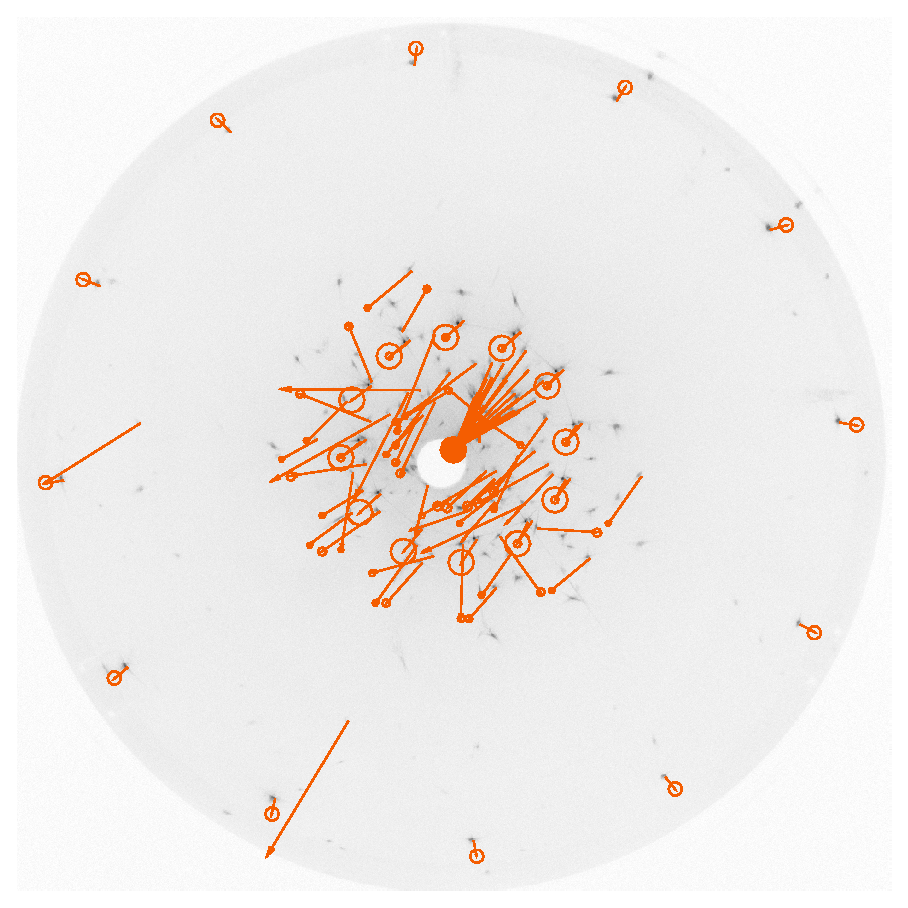
\includegraphics[width=\textwidth]{kores_faze_1.eps}
    \caption[Vzdálenost obrazu korespondujících svazků - fáze 0.]{Vzdálenost obrazu korespondujících svazků po optimalizaci náklonu a rotace kamene \textit{viva12} podle korespondencí třídy \textbf{1A}. Kružnice znázorňují simulované svazky. Čím vyšší je zářivý tok svazku, tím vyšší je poloměr kružnice. Vektory směřují od obrazu pozorovaného svazku k obrazu korespondujícího simulovaného svazku. Modrou barvou jsou zobrazeny volné simulované svazky.}
 \label{fig: kores_faze_0}
 \end{figure}

 
 \begin{figure}[htbp]
    \centering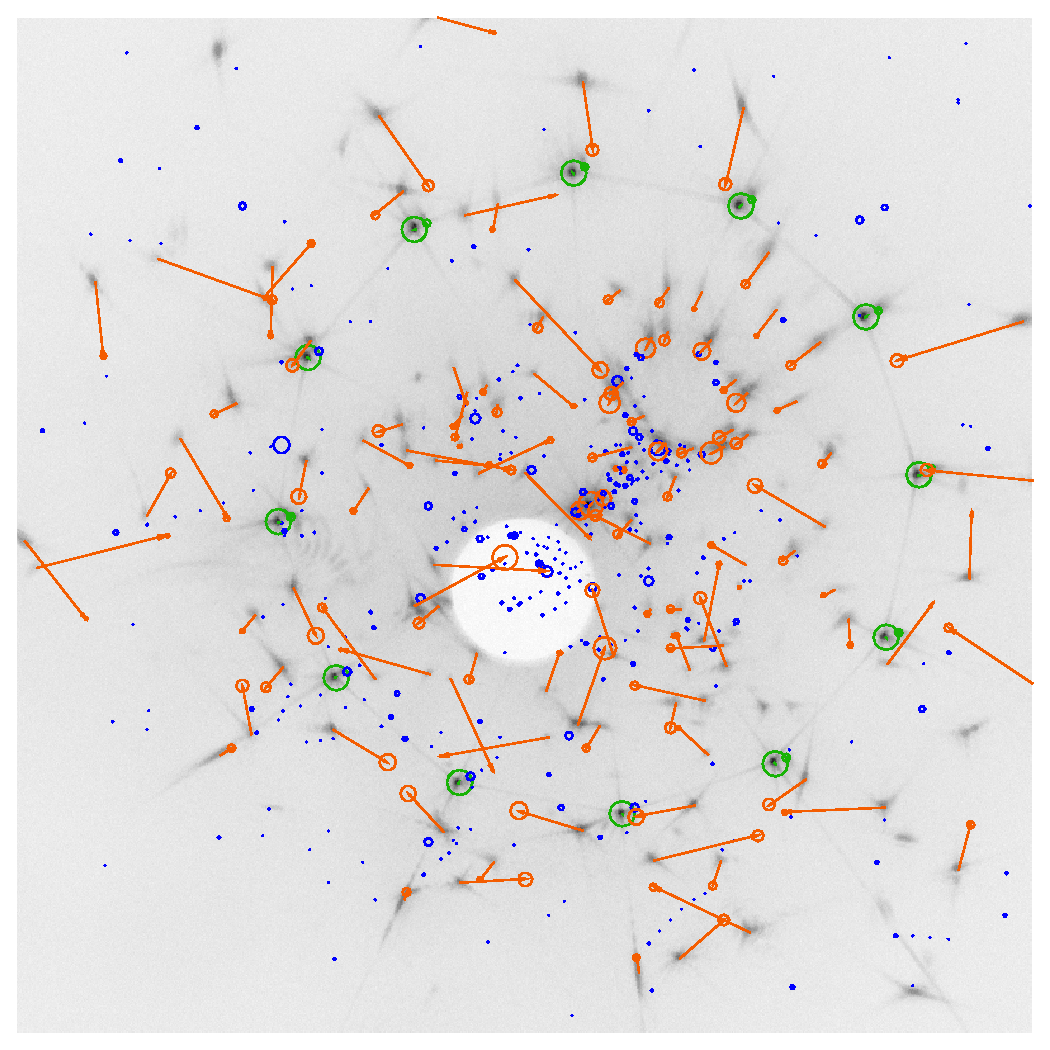
\includegraphics[width=\textwidth]{kores_faze_3.eps}
    \caption[Vzdálenost obrazu korespondujících svazků - fáze 1.]{Detail na střední část snímku \ref{fig: kores_faze_0}. Vzdálenost obrazu korespondujících svazků po optimalizaci náklonu faset podle korespondencí, které lze spolehlivě nalézt. Zelenou barvou jsou zobrazeny korespondence použité při optimalizaci parametrů kamene. Modrou barvou jsou zobrazeny simulované svazky, pro které nebyl nalezen korespondující pozorovaný svazek.}
 \label{fig: kores_faze_1}
 \end{figure}
 
  \begin{figure}[htbp]
    \centering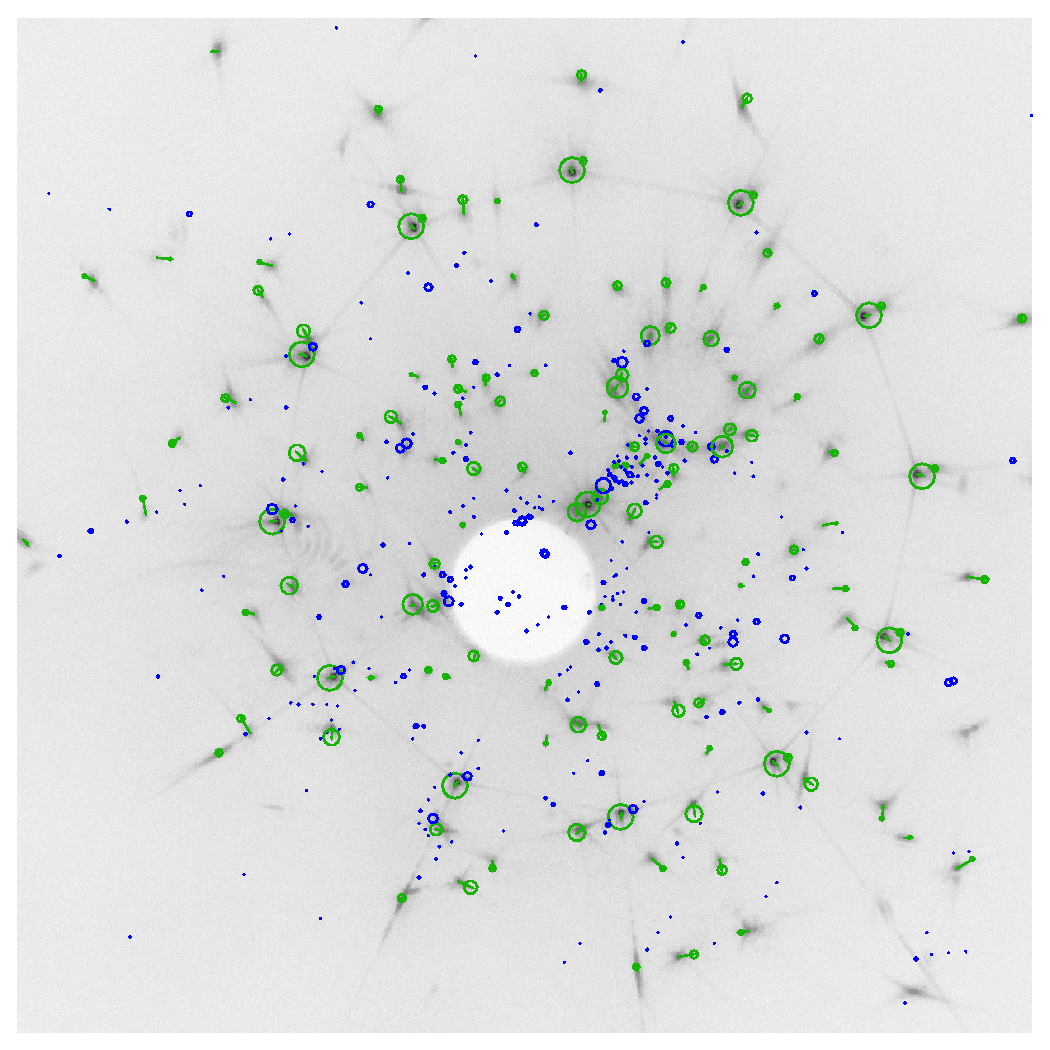
\includegraphics[width=\textwidth]{kores_faze_4.eps}
    \caption[Vzdálenost obrazu korespondujících svazků - konečná fáze.]{Detail na střední část snímku \ref{fig: kores_faze_0}. Vzdálenost obrazu korespondujících svazků po optimalizaci náklonu faset podle všech korespondujících svazků. Zelená barva: korespondující dvojice svazků. Modrá barva: volné simulované svazky.}
 \label{fig: kores_faze_2}
 \end{figure}
 
 \clearpage